\documentclass[conference]{IEEEtran}
\IEEEoverridecommandlockouts

% ---------------------------------------------------------------------------
% Packages
% ---------------------------------------------------------------------------
\usepackage{cite}
\usepackage{amsmath,amssymb,amsfonts}
\usepackage{algorithm}
\usepackage{algorithmic}
\usepackage{graphicx}
\usepackage{textcomp}
\usepackage{xcolor}
\usepackage{booktabs}
\usepackage{multirow}
\usepackage{listings}
\usepackage{tikz}
\usetikzlibrary{arrows.meta,positioning,fit,backgrounds,shapes.geometric}
\usepackage[hidelinks]{hyperref}
\usepackage{balance}

\def\BibTeX{{\rm B\kern-.05em{\sc i\kern-.025em b}\kern-.08em
    T\kern-.1667em\lower.7ex\hbox{E}\kern-.125emX}}


% TypeScript listing style
\lstdefinelanguage{TypeScript}{
  keywords={export,async,function,const,let,await,return,if,throw,new,
            import,from,interface,type,typeof,undefined,null,true,false},
  sensitive=true,
  comment=[l]{//},
  morecomment=[s]{/*}{*/},
  morestring=[b]',
  morestring=[b]",
  morestring=[b]`
}
\lstset{
  language=TypeScript,
  basicstyle=\ttfamily\scriptsize,
  keywordstyle=\bfseries,
  commentstyle=\itshape\color{gray},
  stringstyle=\color{black!75},
  columns=fullflexible,
  keepspaces=true,
  breaklines=true,
  frame=tb,
  framesep=3pt,
  numbers=none,
  numberstyle=\tiny\color{gray},
  xleftmargin=0pt,
  numbersep=4pt,
  captionpos=b
}

\begin{document}

\title{GrindFlow: A Privacy-Preserving, Syllabus-Grounded Peer Learning Platform Powered by a Locally Hosted Large Language Model}

\author{
\IEEEauthorblockN{Purav Bhatt}
\IEEEauthorblockA{\textit{Department of Artificial Intelligence and Data Science}\\
\textit{Dr. Akhilesh Das Gupta Institute of Professional Studies (ADGIPS)}\\
\textit{(Affiliated to Guru Gobind Singh Indraprastha University)}\\
FC-26, Shastri Park, New Delhi 110053, India\\
pbhatt340@gmail.com}
}

\maketitle

% ---------------------------------------------------------------------------
\begin{abstract}
Students increasingly study from peer-authored notes, yet such material varies
widely in quality and is rarely mapped against the official curriculum. General
purpose cloud large language models (LLMs) can critique notes and generate
practice material, but they are not aware of an institution's syllabus,
they send student documents to third-party servers, and their free tiers impose
request quotas that cap concurrency. We present \emph{GrindFlow}, a full-stack
peer learning platform that combines document management, a public notes
library, chat-based study rooms, and three AI services (note scoring,
study-flow generation, and quiz generation). We then propose a design in
which all three are served by a \emph{Syllabus-grounded Local Inference
Engine} (SLIE) instead of a cloud API. SLIE couples a 4-bit quantized open-weight 7--8B instruction-tuned model,
domain-adapted with QLoRA on syllabus-derived instruction data, with a
hierarchical syllabus knowledge base (degree $\rightarrow$ year $\rightarrow$
subject $\rightarrow$ unit $\rightarrow$ topic) queried through hybrid lexical and
dense retrieval. Grammar-constrained decoding guarantees schema-valid JSON, so
the fragile regular-expression recovery used with the cloud model is no longer
needed. We formalize a syllabus-coverage score for notes, a validated
prerequisite-graph construction for study flows, and a verifier-filtered
pipeline for multiple-choice question generation. We analyze the memory and
throughput envelope of the deployment, showing that the complete model plus
four concurrent 8K-token contexts fits in under 10\,GB of accelerator memory,
and we specify an evaluation protocol for comparing the design against the
cloud baseline it replaces. This paper contributes the design and its
analysis; empirical evaluation is left to future work.
\end{abstract}

\begin{IEEEkeywords}
large language models, retrieval-augmented generation, educational technology,
local inference, quantization, automatic question generation, peer learning,
privacy
\end{IEEEkeywords}

% ---------------------------------------------------------------------------
\section{Introduction}

Peer-shared lecture notes are a primary study resource for many undergraduate
students, particularly in the weeks before examinations. Their quality is
uneven. Notes may omit syllabus units, repeat the same topic many times, or
cover material that is not examinable. Students have no cheap way to tell
which of several available notes best matches what they will be assessed on.

LLMs offer an obvious remedy. They can summarize, critique, and generate
retrieval practice, which is among the most effective learning techniques
known~\cite{roediger2006test,dunlosky2013improving}. The first
production version of GrindFlow used a hosted model (Google Gemini~2.5
Flash/Flash-Lite) for exactly these tasks. Operating it exposed four
structural problems:

\begin{enumerate}
\item \textbf{No curriculum awareness.} The cloud model judges a document
against its own general prior rather than the institution's syllabus. The
resulting score measures how good the notes are in general, not how useful
they are for a particular course.
\item \textbf{Data exposure.} Every analysis transmits the full extracted
text of a student's document to a third-party endpoint. This is a concern
under data-protection regimes such as the GDPR~\cite{gdpr2016} and India's
DPDP Act~\cite{dpdp2023}.
\item \textbf{Quota-bound concurrency.} The free tier allowed roughly
15~requests per minute in total. The application had to add a per-user
token-bucket limiter (burst~3, 6~requests/min) and a multi-model retry
cascade. The code's own comments size this for only three or four users
sharing the quota.
\item \textbf{Unstructured output.} The model returned free text that was
supposed to contain JSON. The server had to strip Markdown fences, extract
substrings between the first ``\{'' and the last ``\}'', and fall back to a
sentinel score of~0 when parsing failed.
\end{enumerate}

This paper redesigns GrindFlow's AI layer around a locally hosted model that
\emph{contains the syllabus}, both through parametric adaptation and through
an explicit, queryable knowledge base. The platform described in
Section~\ref{sec:system} is implemented and deployed. The local inference
engine and the algorithms of Sections~\ref{sec:slie}--\ref{sec:features}
are a proposed design, analyzed but not yet empirically evaluated. The
contributions are:

\begin{itemize}
\item A complete system architecture for a peer learning platform
(Section~\ref{sec:system}) built on Next.js, serverless PostgreSQL with the
Drizzle ORM, Clerk authentication, and UploadThing storage, together with its
relational data model.
\item SLIE (Section~\ref{sec:slie}), a drop-in replacement for the cloud LLM
client. It combines a QLoRA-adapted quantized model, hybrid syllabus
retrieval scoped by curriculum metadata, and schema-constrained decoding, and
it exposes the same function signature as the client it replaces.
\item Three syllabus-grounded algorithms (Section~\ref{sec:features}): a
weighted coverage/redundancy score for notes, a validated prerequisite DAG
for study flows, and verifier-filtered MCQ generation weighted by syllabus
marks.
\item An analytical resource model (memory, throughput, and cost) and an
evaluation protocol
(Sections~\ref{sec:impl}--\ref{sec:eval}) for comparing the local system
against the cloud baseline it replaces.
\end{itemize}

% ---------------------------------------------------------------------------
\section{Related Work}

\subsection{LLMs in Education}
Kasneci \textit{et al.}~\cite{kasneci2023chatgpt} survey the opportunities
and risks of LLMs in education, including hallucination and over-reliance.
Intelligent tutoring systems have a long record of measurable learning
gains~\cite{kulik2016effectiveness}. Automatic question generation (AQG) has
been studied extensively~\cite{kurdi2020systematic}, but most systems
generate questions from a single passage without reference to a curriculum.
GrindFlow uses the syllabus to decide \emph{what} to ask and uses the
student's document to decide \emph{how} the question is phrased.

\subsection{Knowledge Injection: Retrieval versus Fine-Tuning}
Retrieval-augmented generation (RAG)~\cite{lewis2020rag,gao2023ragsurvey}
conditions generation on retrieved passages. Ovadia
\textit{et al.}~\cite{ovadia2024finetuning} found that RAG consistently
outperforms unsupervised fine-tuning for injecting new factual knowledge.
RAFT~\cite{zhang2024raft} showed that fine-tuning a model \emph{to use}
retrieved domain documents improves on either technique alone. We follow this
hybrid approach. The syllabus knowledge base is the authoritative source of
facts and can be updated without retraining. A low-rank
adapter~\cite{hu2022lora,dettmers2023qlora} teaches the model the
institution's terminology, output schemas, and how to use retrieved syllabus
context.

\subsection{Efficient Local Inference}
Open-weight models such as Llama~3~\cite{dubey2024llama3} and
Qwen2.5~\cite{qwen2024qwen25} reach strong instruction-following quality at
7--8B parameters. Post-training quantization such as
GPTQ~\cite{frantar2023gptq} and AWQ~\cite{lin2024awq}, together with
the k-quant formats of \texttt{llama.cpp}~\cite{llamacpp}, reduces weights to
about 4--5 bits per parameter with modest quality loss. Serving systems such
as vLLM~\cite{kwon2023pagedattention}, \texttt{llama.cpp}, and
Ollama~\cite{ollama} provide batched, OpenAI-compatible inference on a single
GPU.

\subsection{Structured Generation and Evaluation}
Constrained decoding against a grammar or JSON schema~\cite{willard2023outlines}
guarantees syntactically valid output by masking invalid tokens at each step.
For evaluation, LLM-as-a-judge~\cite{zheng2023judging} and
RAGAS~\cite{es2024ragas} provide automated proxies, which we combine with
faculty annotation.

% ---------------------------------------------------------------------------
\section{System Overview}
\label{sec:system}

\subsection{Functional Scope}
GrindFlow provides: (i) authenticated upload and management of PDF notes;
(ii) AI scoring of a document against a stated purpose and, in this work,
against a syllabus unit; (iii) \emph{study flows}, which are a Mermaid
prerequisite diagram plus a narrative study plan; (iv) auto-generated
multiple-choice quizzes; (v) a public library where students publish scored
notes tagged by degree, year, subject, and unit; and (vi) chat rooms with
\texttt{@mention} notifications for peer discussion.

\subsection{Architecture}
Fig.~\ref{fig:arch} shows the deployment. The web tier is a Next.js
App-Router application. A Clerk edge middleware protects
\texttt{/dashboard}, \texttt{/chat}, \texttt{/explore}, and
\texttt{/onboarding}. Every user-scoped API route also calls
\texttt{requireUser()}, which resolves the Clerk identity and lazily creates a
\texttt{user\_profiles} row. Before any AI work, each document-scoped route
checks that the caller owns the document and returns 403 otherwise. Files are
uploaded directly from the browser to UploadThing (PDF only, at most 32\,MB).
The upload-complete callback inserts the \texttt{documents} row. Relational
state lives in Neon serverless PostgreSQL and is accessed through the
type-safe Drizzle ORM.

The change introduced in this paper is the right-hand side of
Fig.~\ref{fig:arch}. The external Gemini endpoint is removed. AI routes call
an \emph{inference gateway} inside the institution's network. The gateway
performs syllabus retrieval and forwards a constrained request to a local
model server.

\begin{figure*}[t]
\centering
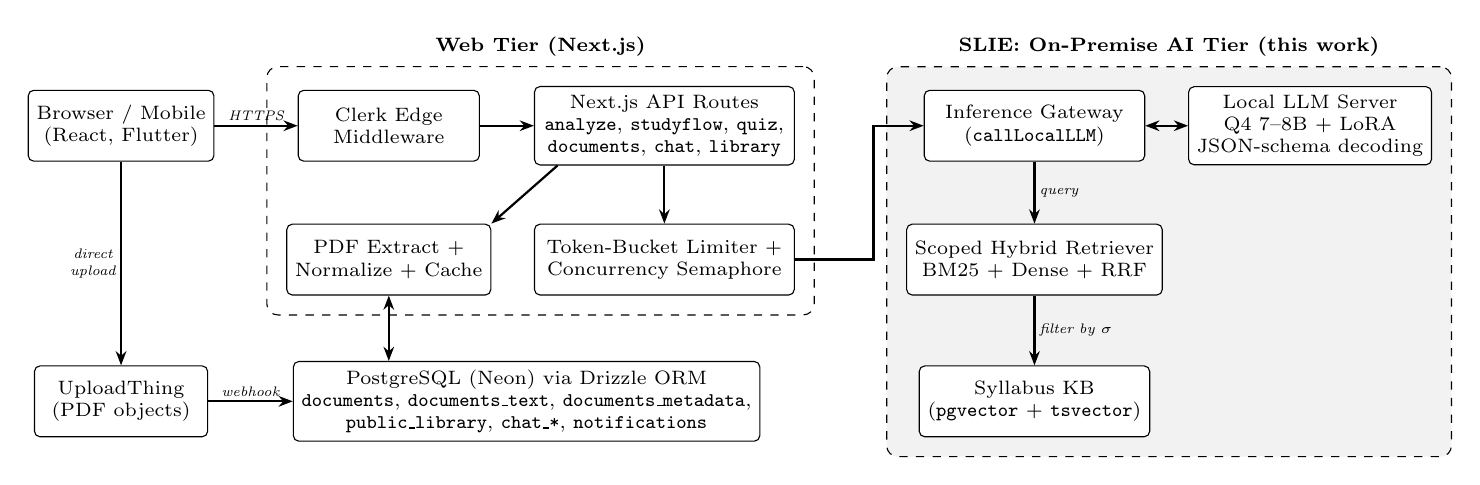
\begin{tikzpicture}[
  font=\scriptsize,
  box/.style={draw, rounded corners=2pt, align=center, minimum height=0.9cm,
              inner sep=3pt, fill=white},
  grp/.style={draw, dashed, rounded corners=4pt, inner sep=7pt},
  arr/.style={-{Stealth[length=1.8mm]}, thick},
  darr/.style={{Stealth[length=1.8mm]}-{Stealth[length=1.8mm]}, thick},
  lbl/.style={font=\tiny\itshape, align=center, inner sep=1.5pt}
]
% Row 1
\node[box, minimum width=2.2cm] (client) at (0,0)   {Browser / Mobile\\(React, Flutter)};
\node[box, minimum width=2.3cm] (mw)     at (3.4,0) {Clerk Edge\\Middleware};
\node[box, minimum width=3.3cm] (api)    at (6.9,0) {Next.js API Routes\\\texttt{analyze}, \texttt{studyflow}, \texttt{quiz},\\\texttt{documents}, \texttt{chat}, \texttt{library}};
\node[box, minimum width=2.8cm] (gw)     at (11.6,0) {Inference Gateway\\(\texttt{callLocalLLM})};
\node[box, minimum width=2.7cm] (llm)    at (15.1,0) {Local LLM Server\\Q4 7--8B + LoRA\\JSON-schema decoding};
% Row 2
\node[box, minimum width=2.3cm] (pre) at (3.4,-1.7)  {PDF Extract +\\Normalize + Cache};
\node[box, minimum width=3.3cm] (rl)  at (6.9,-1.7)  {Token-Bucket Limiter +\\Concurrency Semaphore};
\node[box, minimum width=2.8cm] (ret) at (11.6,-1.7) {Scoped Hybrid Retriever\\BM25 + Dense + RRF};
% Row 3
\node[box, minimum width=2.2cm] (ut)  at (0,-3.5)    {UploadThing\\(PDF objects)};
\node[box, minimum width=5.6cm] (pg)  at (5.15,-3.5) {PostgreSQL (Neon) via Drizzle ORM\\\texttt{documents}, \texttt{documents\_text}, \texttt{documents\_metadata},\\\texttt{public\_library}, \texttt{chat\_*}, \texttt{notifications}};
\node[box, minimum width=2.8cm] (kb)  at (11.6,-3.5) {Syllabus KB\\(\texttt{pgvector} + \texttt{tsvector})};

\begin{scope}[on background layer]
\node[grp, fit=(mw)(api)(pre)(rl), label={[font=\scriptsize\bfseries]above:Web Tier (Next.js)}] {};
\node[grp, fit=(gw)(llm)(ret)(kb), fill=gray!10, label={[font=\scriptsize\bfseries]above:SLIE: On-Premise AI Tier (this work)}] {};
\end{scope}

\draw[arr] (client) -- node[lbl, above]{HTTPS} (mw);
\draw[arr] (mw) -- (api);
\draw[arr] (api) -- (rl);
\draw[arr] ([xshift=3mm]api.south west) -- (pre.north east);
\draw[darr] (pre.south) -- (pre.south |- pg.north);
\draw[arr] (client) -- node[lbl, left]{direct\\upload} (ut);
\draw[arr] (ut) -- node[lbl, above]{webhook} (pg);
\draw[arr] (rl.east) -- ++(1.0,0) |- (gw.west);
\draw[arr] (gw) -- node[lbl, right]{query} (ret);
\draw[arr] (ret) -- node[lbl, right]{filter by $\sigma$} (kb);
\draw[darr] (gw) -- (llm);
\end{tikzpicture}
\caption{GrindFlow deployment architecture. The shaded region is the
Syllabus-grounded Local Inference Engine (SLIE), which replaces the external
cloud LLM endpoint. Document text never leaves the institutional boundary for
inference.}
\label{fig:arch}
\end{figure*}

\subsection{Data Model}
Table~\ref{tab:schema} summarizes the relational schema. Extraction results
are cached per document in \texttt{documents\_text} in three forms: raw text,
normalized text, and a truncated \texttt{short\_text} sized for prompts. This
makes each PDF parse a one-time cost shared by all three AI features. AI
outputs are persisted in \texttt{documents\_metadata}. Published notes carry
curriculum metadata (\texttt{degree}, \texttt{year}, \texttt{subject},
\texttt{unit}) in \texttt{public\_library}. These same keys are the scope
under which SLIE retrieves syllabus context. The syllabus tables introduced
by this work are listed in the lower half of the table.

\begin{table}[t]
\caption{Relational Schema (Existing and Proposed)}
\label{tab:schema}
\centering
\footnotesize
\setlength{\tabcolsep}{3pt}
\begin{tabular}{@{}p{3.0cm}p{5.1cm}@{}}
\toprule
\textbf{Table} & \textbf{Key columns / purpose} \\
\midrule
\multicolumn{2}{@{}l}{\textit{Existing (deployed)}}\\
\texttt{user\_profiles} & Clerk id (PK), unique \texttt{username} \\
\texttt{documents} & owner, file name, storage key, URL \\
\texttt{documents\_text} & raw, normalized, short text (extraction cache) \\
\texttt{documents\_metadata} & \texttt{ai\_rating}, \texttt{ai\_critique} \\
\texttt{public\_library} & subject, unit, year, degree, score, verdict, focus/repetitive topics, plan \\
\texttt{chatrooms} & study rooms (public/private) \\
\texttt{chatroom\_members} & room membership \\
\texttt{chat\_messages} & messages, polled by timestamp cursor \\
\texttt{notifications} & \texttt{@mention} alerts, read state \\
\midrule
\multicolumn{2}{@{}l}{\textit{Proposed (SLIE syllabus KB)}}\\
\texttt{syl\_subjects} & code, name, degree, year, semester, version \\
\texttt{syl\_units} & subject FK, unit no., title, marks weightage $w$ \\
\texttt{syl\_topics} & unit FK, name, outcome text, Bloom level, \texttt{vector(384)} \\
\texttt{syl\_prereqs} & (topic, prerequisite topic) edges \\
\texttt{syl\_chunks} & unit FK, reference text, \texttt{vector(384)}, \texttt{tsvector} \\
\bottomrule
\end{tabular}
\end{table}

% ---------------------------------------------------------------------------
\section{Syllabus-Grounded Local Inference Engine}
\label{sec:slie}

\subsection{Syllabus Knowledge Base}
The syllabus is modeled as a hierarchy
$\mathcal{S} = \{\text{degree} \rightarrow \text{year} \rightarrow
\text{subject} \rightarrow \text{unit} \rightarrow \text{topic}\}$.
Each unit $u$ carries a marks weightage $w_u$, and each topic $t$ carries a
learning-outcome statement and a Bloom's taxonomy level~\cite{anderson2001taxonomy}.
Prerequisite edges between topics form a directed graph $G_{\mathcal{S}}$.
Faculty author the edges, or they are bootstrapped from the order of units in
the syllabus and then reviewed. Official syllabus documents, reference-book
tables of contents, and faculty-provided unit notes are ingested, split into
chunks of about 400 tokens with 15\% overlap along heading boundaries, and
indexed twice. Lexical retrieval uses a PostgreSQL \texttt{tsvector}
(BM25-style ranking~\cite{robertson2009bm25}). Dense retrieval uses 384-dimensional
sentence embeddings~\cite{reimers2019sbert,xiao2024cpack} stored with
\texttt{pgvector} under an HNSW index~\cite{malkov2020hnsw}. Because the KB
lives in the same PostgreSQL instance as the application data, retrieval can
join directly on curriculum metadata.

\subsection{Scoped Hybrid Retrieval}
\label{sec:retrieval}
Given a query $q$ and a curriculum scope
$\sigma = (\text{degree}, \text{year}, \text{subject}, \text{unit})$, the
retriever first filters candidate chunks to $\sigma$. This prevents
cross-course contamination, for example ``normalization'' in a database
course versus a statistics course. It then fuses the lexical ranking
$r_{\text{lex}}$ and the dense ranking $r_{\text{den}}$ with reciprocal rank
fusion~\cite{cormack2009rrf}:
\begin{equation}
\mathrm{RRF}(c) = \sum_{r \in \{r_{\text{lex}}, r_{\text{den}}\}}
\frac{1}{k + r(c)}, \qquad k = 60.
\label{eq:rrf}
\end{equation}
The top-$K$ chunks ($K{=}6$ by default) are prepended to the prompt inside an
explicit \texttt{<syllabus>} block. When the user has not tagged a document,
$\sigma$ is inferred by classifying the document's first 2{,}000 characters
against subject centroids in embedding space, and the student confirms the
result.

\subsection{Model and Domain Adaptation}
The reference deployment uses an open-weight 7--8B instruction-tuned model
(Llama-3.1-8B-Instruct~\cite{dubey2024llama3}; Qwen2.5-7B-Instruct~\cite{qwen2024qwen25}
as an alternative). It is adapted with QLoRA~\cite{dettmers2023qlora}
(rank $r{=}16$, $\alpha{=}32$, all attention and MLP projections) on an
instruction set synthesized from the KB: topic explanations, outcome-to-topic
mapping, critiques of synthetic notes with deliberately missing units, and
MCQs with keys. Following RAFT~\cite{zhang2024raft}, a fraction of training
examples include retrieved context mixed with distractor chunks, so the
adapter learns to rely on relevant syllabus passages and ignore irrelevant
ones. The KB, not the adapter, is the source of truth. When the syllabus is
revised, only the KB is re-indexed. The adapter is retrained only when the
output schemas or institutional terminology change.

After merging, the model is quantized to a 4-bit k-quant GGUF format
(Q4\_K\_M, about 4.85 bits per weight) and served by the \texttt{llama.cpp}
HTTP server with $N$ parallel decoding slots and continuous batching.
Ollama~\cite{ollama} or vLLM~\cite{kwon2023pagedattention} with
AWQ~\cite{lin2024awq} weights can be used interchangeably, since all three
expose an OpenAI-compatible endpoint.

\subsection{Schema-Constrained Decoding}
Each AI route declares a JSON Schema for its output, for example
\texttt{\{score:int[0,100], verdict:string, rationale:string,
focus\_topics:string[], \ldots\}}. The server compiles the schema to a
grammar and masks invalid tokens at every step~\cite{willard2023outlines}.
Parsing therefore cannot fail. This removes the code path that
previously returned \texttt{\{score:0, verdict:"unable\_to\_parse"\}} and
silently stored a zero rating.

\subsection{Drop-in Client Interface}
To minimize change in the application, SLIE exposes \texttt{callLocalLLM},
which keeps the call shape of the former \texttt{callGemini(system, user,
opts)} and adds two optional fields: the curriculum scope and the output
schema (Listing~\ref{lst:client}). The retry strategy also changes. The cloud
client retried on HTTP~429/503 and cascaded across model variants with
back-off delays of 0.5, 1.2, 3, and 6\,s. A local server under the
application's control does not throttle by quota. Overload is instead handled
before the request is sent, by a counting semaphore sized to the server's
$N$ slots. Requests that cannot obtain a slot within a short deadline return
HTTP~503 with a \texttt{Retry-After} header.

\begin{lstlisting}[caption={Proposed SLIE client (abridged). The signature matches the replaced cloud client, so each route handler changes by one import.},label={lst:client},float=t]
export async function callLocalLLM(
  system: string, user: string, o: LocalOpts = {}
): Promise<string> {
  const ctx = o.scope
    ? await retrieveSyllabus(user, o.scope, 6) : []
  const release = await slots.acquire(o.queueMs ?? 4000)
  try {
    const body = {
      model: LOCAL_MODEL,
      temperature: o.temperature ?? 0.2,
      messages: [
        { role: 'system', content: system },
        { role: 'user',
          content: renderSyllabus(ctx) + user },
      ],
      response_format: o.schema &&
        { type: 'json_object', schema: o.schema },
    }
    const res = await withTimeout(fetch(CHAT_URL, {
      method: 'POST',
      headers: { 'Content-Type': 'application/json' },
      body: JSON.stringify(body),
    }), o.timeoutMs ?? 30000)
    if (!res.ok)
      throw new LocalLLMUnavailableError(res.status)
    const data = await res.json()
    return data.choices[0].message.content
  } finally { release() }
}
\end{lstlisting}

% ---------------------------------------------------------------------------
\section{Syllabus-Grounded AI Features}
\label{sec:features}

\subsection{Document Preprocessing}
Text is extracted from the PDF text layer and normalized by
Algorithm~\ref{alg:norm}, which is implemented in the deployed system. Short
lines of at most 50 characters that occur more than twice are treated as
running headers, footers, or slide titles and dropped. Runs of whitespace and
blank lines are collapsed. The normalized text is cached and truncated to a
per-feature character budget (Table~\ref{tab:budget}).

\begin{algorithm}[t]
\caption{Prompt-Oriented Text Normalization}
\label{alg:norm}
\begin{algorithmic}[1]
\REQUIRE raw text $X$, short-line length $\ell{=}50$, repeat limit $m{=}2$
\ENSURE normalized text $Y$
\STATE $seen \leftarrow \emptyset$ (multiset); $K \leftarrow [\,]$
\FORALL{line $x$ in $X$}
  \STATE $x \leftarrow \mathrm{trim}(x)$
  \IF{$x = \varepsilon$} \STATE \textbf{continue} \ENDIF
  \IF{$|x| \le \ell$}
    \STATE $seen[\mathrm{lower}(x)] \mathrel{+}= 1$
    \IF{$seen[\mathrm{lower}(x)] > m$} \STATE \textbf{continue} \ENDIF
  \ENDIF
  \STATE append $x$ to $K$
\ENDFOR
\STATE $Y \leftarrow \mathrm{join}(K, \texttt{\textbackslash n})$
\STATE collapse runs of $\ge 2$ spaces/tabs to one space
\STATE collapse runs of $\ge 3$ newlines to two
\RETURN $Y$
\end{algorithmic}
\end{algorithm}

\subsection{Note Scoring by Syllabus Coverage}
Let unit $u$ have topics $T_u = \{t_1,\dots,t_m\}$ with weights $w_i$
(topic-level marks weightage, uniform within a unit by default). Let the
document be chunked into $D = \{d_1,\dots,d_n\}$, and let $e(\cdot)$ denote
the unit-normalized embedding. The coverage of topic $t_i$ is
\begin{equation}
\kappa_i = \max_{1\le j\le n} \; e(t_i)^{\top} e(d_j),
\end{equation}
and the weighted syllabus coverage of the document is
\begin{equation}
C(D,u) = \frac{\sum_{i=1}^{m} w_i \,\mathbf{1}[\kappa_i \ge \tau]}{\sum_{i=1}^{m} w_i}.
\label{eq:cov}
\end{equation}
Redundancy measures how much of the document is concentrated on few topics.
Let $n_i = |\{j : e(t_i)^{\top}e(d_j) \ge \tau\}|$ be the number of chunks
attributed to topic $t_i$. The redundancy is
\begin{equation}
R(D,u) = \frac{1}{n}\sum_{i=1}^{m} \max\!\left(0,\; n_i - \lambda\frac{n}{m}\right),
\label{eq:red}
\end{equation}
which is the fraction of chunks in excess of $\lambda$ times a uniform share.
The local model, conditioned on the retrieved learning outcomes, returns a
rubric quality score $Q \in [0,100]$ covering accuracy, clarity,
organization, and depth. The final score is
\begin{equation}
S = \mathrm{clip}_{[0,100]}\Big(\alpha \cdot 100\,C + (1-\alpha)\,Q - \gamma \cdot 100\,R\Big).
\label{eq:score}
\end{equation}
We use $\alpha{=}0.5$, $\gamma{=}0.2$, $\lambda{=}2$ as defaults and
calibrate $\tau$ on a held-out annotated set (Section~\ref{sec:eval}). The
deployed response schema maps directly onto these quantities.
\texttt{focus\_topics} is the set $\{t_i : \kappa_i < \tau\}$ ordered by
$w_i$, which are the syllabus gaps the student must study elsewhere.
\texttt{repetitive\_topics} is the set
$\{t_i : n_i > \lambda n/m\}$. \texttt{suggested\_plan} is generated by the
model from both lists. Because $C$ and $R$ are computed deterministically
outside the LLM, two of the three terms of the score are reproducible and
explainable. This addresses the main criticism of opaque LLM
grading~\cite{zheng2023judging}.

\subsection{Validated Study Flows}
The deployed system asks the model for a Mermaid \texttt{flowchart TD} of at
most 20 nodes and a 300--500 word study plan, issued as two parallel
requests. Without grounding, the generated graphs can contain cycles,
invented topics, or missing prerequisites. SLIE adds a validation stage
(Algorithm~\ref{alg:flow}). Nodes are canonicalized against $T_u$ by
embedding similarity. Edges from the syllabus graph $G_{\mathcal{S}}$ are
merged in. Cycles are broken by discarding model-proposed edges before
syllabus edges. A study order is produced by Kahn's topological sort with
ties broken by weight. The validated graph is then re-serialized to Mermaid,
which guarantees that the client-side renderer receives syntactically valid
input.

\begin{algorithm}[t]
\caption{Syllabus-Validated Study-Flow Construction}
\label{alg:flow}
\begin{algorithmic}[1]
\REQUIRE model graph $G_M=(V_M,E_M)$, unit topics $T_u$, syllabus edges $E_{\mathcal{S}}$, threshold $\tau$
\ENSURE DAG $G^\ast$ and study order $\pi$
\STATE $\phi(v) \leftarrow \arg\max_{t \in T_u} e(v)^\top e(t)$ if the max $\ge \tau$, else $\bot$
\STATE $V \leftarrow \{\phi(v) : v \in V_M, \phi(v)\neq\bot\}$
\STATE $E \leftarrow \{(t,t') \in E_{\mathcal{S}} : t,t' \in V\}$ \COMMENT{trusted}
\FORALL{$(v,v') \in E_M$ with $\phi(v),\phi(v')\neq\bot$}
  \IF{adding $(\phi(v),\phi(v'))$ to $E$ keeps $(V,E)$ acyclic}
    \STATE $E \leftarrow E \cup \{(\phi(v),\phi(v'))\}$
  \ENDIF
\ENDFOR
\STATE $\pi \leftarrow$ \textsc{KahnTopoSort}$(V,E)$, ties by descending $w$
\RETURN $G^\ast=(V,E)$, $\pi$
\end{algorithmic}
\end{algorithm}

\subsection{Syllabus-Weighted, Verified Quiz Generation}
The deployed quiz route first narrows the document to lines matching the
student's keywords. It keeps the slice only if at least five lines match,
truncates to 5{,}000 characters (fast mode, 6~questions) or 18{,}000
characters (10~questions), and retries once with a broader 9{,}000/14{,}000
character window if no question parses. SLIE keeps this flow and adds three
steps:
\begin{enumerate}
\item \textbf{Blueprinting.} The $q$ questions are allocated across topics in
proportion to $w_i$ and across Bloom levels according to the topic's target
outcome. This mirrors how examination blueprints are drawn up.
\item \textbf{Grounded generation.} Each item is generated with the relevant
document passage and the topic's syllabus chunks in context, under a schema
that requires exactly four options and \texttt{correctIndex}~$\in\{0,1,2,3\}$.
\item \textbf{Verification.} A second, independent call answers the item
\emph{without} the key. The item is kept only if the verifier's answer
matches the key and every pair of distractors has cosine similarity below
$0.9$. Rejected slots are regenerated once.
\end{enumerate}

\subsection{Public Library Tagging}
When a student publishes a scored document, the subject and unit are
pre-filled by the scope classifier of Section~\ref{sec:retrieval}. The stored
\texttt{focus\_topics} and \texttt{repetitive\_topics} then refer to
canonical syllabus topic names rather than free text, so the library can be
filtered by topic as well as by subject.

% ---------------------------------------------------------------------------
\section{Implementation and Resource Analysis}
\label{sec:impl}

\subsection{Prompt Budgets}
Table~\ref{tab:budget} lists the context budgets that the deployed routes
enforce. Assuming about 4 characters per token for English technical prose,
the largest prompt (note scoring) is about 4.5K tokens of document text. Six
retrieved syllabus chunks add about 2.4K tokens and system instructions add
fewer than 0.5K, so an 8{,}192-token context window suffices for every
feature.

\begin{table}[t]
\caption{Per-Feature Budgets Enforced by the Application}
\label{tab:budget}
\centering
\setlength{\tabcolsep}{4pt}
\begin{tabular}{@{}lcccc@{}}
\toprule
\textbf{Feature} & \textbf{Doc. chars} & \textbf{$\approx$Tokens} & \textbf{Timeout} & \textbf{Attempts}\\
\midrule
Note scoring    & 18{,}000 & 4{,}500 & 22\,s & 3 \\
Study flow (each of 2) & 10{,}000 & 2{,}500 & 15\,s & 2 \\
Quiz, fast (6 Q)  & 5{,}000  & 1{,}250 & 18\,s & 2 (+1 retry)\\
Quiz, full (10 Q) & 18{,}000 & 4{,}500 & 22\,s & 2 (+1 retry)\\
\bottomrule
\end{tabular}
\end{table}

\subsection{Accelerator Memory Envelope}
Memory is dominated by the weights and the key--value (KV) cache. For a model
with $L$ layers, $H_{kv}$ KV heads of dimension $d_h$, stored at $b$ bytes
per element, the KV cache per token is
\begin{equation}
M_{\text{KV}} = 2\,L\,H_{kv}\,d_h\,b .
\end{equation}
For Llama-3.1-8B ($L{=}32$, $H_{kv}{=}8$, $d_h{=}128$, FP16) this is
131{,}072\,B (128\,KiB) per token, or 1\,GiB per 8K-token slot. For
Qwen2.5-7B ($L{=}28$, $H_{kv}{=}4$) it is 56\,KiB per token.
Table~\ref{tab:mem} gives the resulting totals. With Q4\_K\_M weights and four
concurrent 8K slots, the 8B model needs about 9.2\,GB and the 7B model about
6.5\,GB, excluding small runtime buffers. Both fit on a single 12\,GB
consumer GPU. The same budget holds on a 16\,GB unified-memory laptop for
single-user development.

\begin{table}[t]
\caption{Analytical Memory Footprint (GB, $10^9$ bytes)}
\label{tab:mem}
\centering
\setlength{\tabcolsep}{4pt}
\begin{tabular}{@{}lccc@{}}
\toprule
\textbf{Component} & \textbf{FP16} & \textbf{Q8\_0} & \textbf{Q4\_K\_M}\\
\midrule
Llama-3.1-8B weights (8.03B) & 16.06 & 8.53 & 4.87 \\
Qwen2.5-7B weights (7.62B)   & 15.24 & 8.10 & 4.62 \\
\midrule
KV, Llama, $4\times$8K slots & \multicolumn{3}{c}{4.29}\\
KV, Qwen,  $4\times$8K slots & \multicolumn{3}{c}{1.88}\\
\midrule
\textbf{Total, Llama Q4 + 4 slots} & \multicolumn{3}{c}{\textbf{9.16}}\\
\textbf{Total, Qwen Q4 + 4 slots}  & \multicolumn{3}{c}{\textbf{6.50}}\\
\bottomrule
\end{tabular}
\end{table}

\subsection{Rate Limiting and Fairness}
The deployed per-user limiter is a token bucket~\cite{tanenbaum2011networks}
with capacity $b{=}3$ and refill $\rho{=}6$ tokens/min, kept separately for
each (user, feature) pair. Over any window of $T$ minutes a user can issue at
most $b + \rho T$ AI requests. With the cloud model, the binding constraint
was the provider's global quota $Q_{\text{prov}}{\approx}15$\,RPM, which
supports only $\lfloor Q_{\text{prov}}/\rho \rfloor = 2$ users at their
sustained maximum. With SLIE the provider quota disappears. The bucket is
kept as a fairness control, and capacity becomes a function of hardware: if
a request occupies a slot for $\bar{s}$ seconds on average, the server
sustains $60N/\bar{s}$ requests per minute. The bucket state is currently held
in process memory, which is correct only for a single application instance.
Horizontal scaling requires moving it to a shared store.

\subsection{Cost Model}
Let $P$ and $G$ be prompt and generated tokens per request. A metered cloud
API costs $P c_{\text{in}} + G c_{\text{out}}$ per request. A local server
with capital cost $C_{\text{hw}}$ amortized over $Y$ years, average power
draw $W$\,kW, and electricity price $p$ per kWh costs
\begin{equation}
c_{\text{local}} = \frac{C_{\text{hw}}}{Y \cdot N_{\text{req/yr}}} +
\frac{W\,\bar{s}}{3600\,N}\,p
\end{equation}
per request. The break-even volume
$N^{\ast}_{\text{req/yr}}$ follows by equating the two. Beyond cost, the
local deployment has no per-request marginal data exposure.

\subsection{Security Considerations}
Uploaded documents are untrusted input placed into prompts, so they are a
vector for prompt injection. SLIE limits the impact in three ways. Document
text is wrapped in explicit delimiters and labeled as data in the system
prompt. Schema-constrained decoding means an injected instruction can at most
alter field \emph{values}, not the response structure or any tool behavior
(the model has no tools). The deterministic coverage terms of
Eq.~\eqref{eq:score} bound how far an injected ``give this a 100'' can move the
final score: by at most $(1-\alpha)\cdot100 = 50$ points. Ownership checks on
every document-scoped route prevent one user from triggering analysis of
another user's file.

% ---------------------------------------------------------------------------
\section{Proposed Evaluation Protocol}
\label{sec:eval}

The protocol below is designed so that each AI feature can be compared against
the cloud baseline it replaces, and so that the contribution of each SLIE
component can be isolated by ablation.

\subsection{Research Questions}
\begin{description}
\item[RQ1] Does syllabus grounding make note scores agree more closely with
faculty judgments of exam usefulness?
\item[RQ2] Are generated quizzes more syllabus-aligned and more often
correct?
\item[RQ3] Do validated study flows recover faculty-authored prerequisite
structure?
\item[RQ4] What latency, reliability, and resource cost does local inference
incur relative to the cloud baseline?
\end{description}

\subsection{Configurations}
\textbf{C0}: production baseline, Gemini~2.5 Flash-Lite with the deployed
prompts. \textbf{C1}: local Q4 model, no retrieval, no adapter.
\textbf{C2}: C1 + scoped hybrid retrieval. \textbf{C3}: C2 + QLoRA adapter
(full SLIE). \textbf{C3$^-$}: C3 without constrained decoding (ablation).

\subsection{Data and Annotation}
The planned corpus consists of student-contributed PDF notes, collected with
informed consent, across several subjects of one degree program, each with its
official syllabus. Two or more faculty members per subject will rate each
document for exam usefulness on a 0--100 scale, author the unit prerequisite
graph, and judge generated MCQs for correctness, syllabus alignment, and
distractor plausibility. Inter-rater agreement will be reported as
Krippendorff's $\alpha$. The coverage threshold $\tau$ and the weights in
Eq.~\eqref{eq:score} will be tuned on a 20\% development split and frozen
before testing, so that test results are not fitted to the test set.

\subsection{Metrics}
RQ1: Spearman $\rho$ and mean absolute error between $S$ and the mean faculty
rating; precision/recall of \texttt{focus\_topics} against faculty-identified
gaps. RQ2: answer-key accuracy, syllabus-alignment rate, verifier rejection
rate. RQ3: edge precision, recall, and F1 against the faculty graph;
cycle rate; Mermaid render-success rate. RQ4: JSON-validity rate, p50/p95
latency, sustained requests/min, peak accelerator memory.

\subsection{Hypotheses}
From the design and prior work on retrieval grounding~\cite{ovadia2024finetuning,zhang2024raft},
we expect the following. (H1) C1 will trail C0 on quality metrics, since a
4-bit 7--8B model has less general knowledge than a hosted model. (H2) Scoped
retrieval (C2) will close or reverse this gap on the syllabus-dependent
metrics (score agreement, gap-topic F1, syllabus alignment, edge F1), because
the model is told what the course examines. (H3) The adapter (C3) will add a
smaller gain, mainly through canonical topic naming that improves the matching
steps of Eq.~\eqref{eq:cov} and Algorithm~\ref{alg:flow}. (H4) C1--C3 will
produce schema-valid output in all cases by construction, and C3$^-$ will not.
(H5) Sustained throughput will follow $60N/\bar{s}$
(Section~\ref{sec:impl}) and will no longer be bounded by a provider quota.
Each hypothesis maps to one research question and is falsifiable with the
metrics above.

\subsection{Threats to Validity}
Faculty ratings of ``usefulness'' are subjective and course-specific.
Embedding-based coverage can reward keyword-dense but shallow notes, which the
rubric term $Q$ is meant to offset. Results from one degree program may not
transfer to curricula with different structure. Self-verification of MCQs
uses the same base model as generation, so correlated errors can pass the
filter. A verifier drawn from a different model family would reduce this risk.

% ---------------------------------------------------------------------------
\section{Discussion and Limitations}

\textit{Why not fine-tuning alone?} Syllabi are revised every year or two,
and a parametric-only model would silently go stale. Retrieval keeps facts
current and citable. The adapter supplies format discipline and institutional
vocabulary, consistent with~\cite{ovadia2024finetuning,zhang2024raft}.

\textit{Residual cloud dependencies.} Moving inference on-premise removes the
largest data flow, but authentication (Clerk), object storage (UploadThing),
and the database (Neon) remain managed services. A fully sovereign deployment
would substitute self-hosted PostgreSQL with \texttt{pgvector}, an
S3-compatible object store, and an OIDC provider. The ORM and route handlers
are agnostic to these choices.

\textit{Extraction.} The PDF parser reads only the embedded text layer.
Scanned or handwritten notes, which are common among students, require an OCR
stage before Algorithm~\ref{alg:norm}.

\textit{Operational limits.} The in-memory rate limiter and the polling-based
chat (\texttt{since}-cursor queries capped at 500 messages) are adequate for
a single instance. Larger deployments need a shared limiter store and a push
channel such as WebSockets or server-sent events.

% ---------------------------------------------------------------------------
\section{Conclusion and Future Work}
We presented GrindFlow, a peer learning platform, and a design that grounds
its AI services in the institution's own syllabus and runs them entirely on a
locally hosted, quantized open-weight model. Explicit curriculum structure
(weightages, learning outcomes, and prerequisite edges) turns three loosely
specified LLM tasks into partly deterministic, auditable computations.
Schema-constrained decoding removes a whole class of parsing failures, and
local serving replaces a hard provider quota with a capacity that grows with
hardware. Our analysis shows that the full stack fits on a single commodity
GPU. Future work includes implementing SLIE in the deployed platform and
carrying out the evaluation of
Section~\ref{sec:eval}, adding OCR for handwritten notes, spaced-repetition
scheduling of missed quiz items, a companion Flutter mobile client, and
on-device inference with sub-3B models for offline study.

\section*{Acknowledgment}
The author thanks Shreya Jha, Devyani Dadawal, Piyush Thakur, and Tushar
Kaushik, who co-developed the GrindFlow platform.

% ---------------------------------------------------------------------------
\begin{thebibliography}{99}
\footnotesize

\bibitem{roediger2006test}
H.~L. Roediger and J.~D. Karpicke, ``Test-enhanced learning: Taking memory
tests improves long-term retention,'' \textit{Psychol. Sci.}, vol.~17, no.~3,
pp.~249--255, 2006.

\bibitem{dunlosky2013improving}
J.~Dunlosky, K.~A. Rawson, E.~J. Marsh, M.~J. Nathan, and D.~T. Willingham,
``Improving students' learning with effective learning techniques: Promising
directions from cognitive and educational psychology,'' \textit{Psychol. Sci.
Public Interest}, vol.~14, no.~1, pp.~4--58, 2013.

\bibitem{gdpr2016}
European Parliament and Council, ``Regulation (EU) 2016/679 (General Data
Protection Regulation),'' \textit{Off. J. Eur. Union}, vol.~L119, pp.~1--88,
2016.

\bibitem{dpdp2023}
Government of India, ``The Digital Personal Data Protection Act, 2023,'' Act
No.~22 of 2023, Ministry of Law and Justice, New Delhi, 2023.

\bibitem{kasneci2023chatgpt}
E.~Kasneci \textit{et al.}, ``ChatGPT for good? On opportunities and
challenges of large language models for education,'' \textit{Learn. Individ.
Differ.}, vol.~103, Art.~no.~102274, 2023.

\bibitem{kulik2016effectiveness}
J.~A. Kulik and J.~D. Fletcher, ``Effectiveness of intelligent tutoring
systems: A meta-analytic review,'' \textit{Rev. Educ. Res.}, vol.~86, no.~1,
pp.~42--78, 2016.

\bibitem{kurdi2020systematic}
G.~Kurdi, J.~Leo, B.~Parsia, U.~Sattler, and S.~Al-Emari, ``A systematic
review of automatic question generation for educational purposes,''
\textit{Int. J. Artif. Intell. Educ.}, vol.~30, no.~1, pp.~121--204, 2020.

\bibitem{lewis2020rag}
P.~Lewis \textit{et al.}, ``Retrieval-augmented generation for
knowledge-intensive NLP tasks,'' in \textit{Proc. Adv. Neural Inf. Process.
Syst. (NeurIPS)}, vol.~33, 2020, pp.~9459--9474.

\bibitem{gao2023ragsurvey}
Y.~Gao \textit{et al.}, ``Retrieval-augmented generation for large language
models: A survey,'' arXiv:2312.10997, 2023.

\bibitem{ovadia2024finetuning}
O.~Ovadia, M.~Brief, M.~Mishaeli, and O.~Elisha, ``Fine-tuning or retrieval?
Comparing knowledge injection in LLMs,'' in \textit{Proc. Conf. Empirical
Methods Natural Lang. Process. (EMNLP)}, 2024, pp.~237--250.

\bibitem{zhang2024raft}
T.~Zhang \textit{et al.}, ``RAFT: Adapting language model to domain specific
RAG,'' in \textit{Proc. Conf. Lang. Model. (COLM)}, 2024.

\bibitem{hu2022lora}
E.~J. Hu \textit{et al.}, ``LoRA: Low-rank adaptation of large language
models,'' in \textit{Proc. Int. Conf. Learn. Represent. (ICLR)}, 2022.

\bibitem{dettmers2023qlora}
T.~Dettmers, A.~Pagnoni, A.~Holtzman, and L.~Zettlemoyer, ``QLoRA: Efficient
finetuning of quantized LLMs,'' in \textit{Proc. Adv. Neural Inf. Process.
Syst. (NeurIPS)}, vol.~36, 2023.

\bibitem{dubey2024llama3}
A.~Dubey \textit{et al.}, ``The Llama 3 herd of models,''
arXiv:2407.21783, 2024.

\bibitem{qwen2024qwen25}
Qwen Team, ``Qwen2.5 technical report,'' arXiv:2412.15115, 2024.

\bibitem{frantar2023gptq}
E.~Frantar, S.~Ashkboos, T.~Hoefler, and D.~Alistarh, ``GPTQ: Accurate
post-training quantization for generative pre-trained transformers,'' in
\textit{Proc. Int. Conf. Learn. Represent. (ICLR)}, 2023.

\bibitem{lin2024awq}
J.~Lin \textit{et al.}, ``AWQ: Activation-aware weight quantization for
on-device LLM compression and acceleration,'' in \textit{Proc. Mach. Learn.
Syst. (MLSys)}, 2024.

\bibitem{llamacpp}
G.~Gerganov \textit{et al.}, ``llama.cpp: LLM inference in C/C++,'' GitHub
repository. [Online]. Available: https://github.com/ggml-org/llama.cpp

\bibitem{kwon2023pagedattention}
W.~Kwon \textit{et al.}, ``Efficient memory management for large language
model serving with PagedAttention,'' in \textit{Proc. 29th ACM Symp.
Operating Syst. Principles (SOSP)}, 2023, pp.~611--626.

\bibitem{ollama}
Ollama, ``Get up and running with large language models locally,'' GitHub
repository. [Online]. Available: https://github.com/ollama/ollama

\bibitem{willard2023outlines}
B.~T. Willard and R.~Louf, ``Efficient guided generation for large language
models,'' arXiv:2307.09702, 2023.

\bibitem{zheng2023judging}
L.~Zheng \textit{et al.}, ``Judging LLM-as-a-judge with MT-Bench and Chatbot
Arena,'' in \textit{Proc. Adv. Neural Inf. Process. Syst. (NeurIPS)},
vol.~36, Datasets and Benchmarks Track, 2023.

\bibitem{es2024ragas}
S.~Es, J.~James, L.~Espinosa-Anke, and S.~Schockaert, ``RAGAS: Automated
evaluation of retrieval augmented generation,'' in \textit{Proc. 18th Conf.
Eur. Chapter Assoc. Comput. Linguist.: Syst. Demonstrations (EACL)}, 2024,
pp.~150--158.

\bibitem{anderson2001taxonomy}
L.~W. Anderson and D.~R. Krathwohl, Eds., \textit{A Taxonomy for Learning,
Teaching, and Assessing: A Revision of Bloom's Taxonomy of Educational
Objectives}. New York, NY, USA: Longman, 2001.

\bibitem{robertson2009bm25}
S.~Robertson and H.~Zaragoza, ``The probabilistic relevance framework: BM25
and beyond,'' \textit{Found. Trends Inf. Retr.}, vol.~3, no.~4,
pp.~333--389, 2009.

\bibitem{reimers2019sbert}
N.~Reimers and I.~Gurevych, ``Sentence-BERT: Sentence embeddings using
Siamese BERT-networks,'' in \textit{Proc. Conf. Empirical Methods Natural
Lang. Process. (EMNLP-IJCNLP)}, 2019, pp.~3982--3992.

\bibitem{xiao2024cpack}
S.~Xiao, Z.~Liu, P.~Zhang, N.~Muennighoff, D.~Lian, and J.-Y. Nie, ``C-Pack:
Packed resources for general Chinese embeddings,'' in \textit{Proc. 47th Int.
ACM SIGIR Conf. Res. Develop. Inf. Retr.}, 2024, pp.~641--649.

\bibitem{malkov2020hnsw}
Y.~A. Malkov and D.~A. Yashunin, ``Efficient and robust approximate nearest
neighbor search using hierarchical navigable small world graphs,''
\textit{IEEE Trans. Pattern Anal. Mach. Intell.}, vol.~42, no.~4,
pp.~824--836, Apr. 2020.

\bibitem{cormack2009rrf}
G.~V. Cormack, C.~L.~A. Clarke, and S.~Buettcher, ``Reciprocal rank fusion
outperforms Condorcet and individual rank learning methods,'' in
\textit{Proc. 32nd Int. ACM SIGIR Conf. Res. Develop. Inf. Retr.}, 2009,
pp.~758--759.

\bibitem{tanenbaum2011networks}
A.~S. Tanenbaum and D.~J. Wetherall, \textit{Computer Networks}, 5th~ed.
Boston, MA, USA: Pearson, 2011.

\end{thebibliography}

\end{document}
